\providecommand{\main}{../main}
\documentclass[\main/main.tex]{subfiles}
\graphicspath{{../images/}}
\begin{document}
\section{
    場の理論(速習)
}
この記事では主に経路積分表示によるEuclid化された場の理論を扱っている。
扱うのはBosonのみで、Fermionの経路積分については説明しない。

% 場の理論の具体的な計算例を全く載せていないので、議論が抽象的すぎるかもしれない。
% そのように思われる場合、補足にある自由場についてのいくつかの計算を見ると良いと思う。
\subsection{
    Euclid空間における場の理論
}
経路積分を用いて、古典統計力学系の連続極限として場の理論を導入しよう。
場の理論の定式化にはいくつか方法があるが、経路積分の方法には
\begin{itemize}
    \item 統計力学と量子論の対応関係が見やすい
    \item 理論の対称性が見やすい
    \item 古典極限をとりやすい
\end{itemize}
などの利点がある。

例えばの格子間隔$a$の格子点$x = an, n ∈ ℤ^d$上にスピン変数$s_n$が定義されていたとする。
系のエネルギーを$E[s]$とすると、分配関数は
\begin{align}
    Z = ∑_{[s]}\e^{-βE[s]}
\end{align}
と書ける。ここで$β$は逆温度であり、$∑_{[s]}$は取りうるあらゆるスピンの配位についての和を表す。
このような格子上で定義された模型において格子間隔$a → 0$の極限をとることで、連続的な場の理論が得られる。
このとき、何を保ちながら極限をとるのかを決めておく必要があるが、この問題については後で考える。

場$ϕ(x)$を時空$ℝ^d$ (Euclid空間)上で定義された実数値をとる関数とする。
\footnote{
    この時点で場がBoson的であることを仮定していることになる。
    Fermionを扱いたい場合はGrassmann数を用いる。
}
この仮定は議論を単純にするためで、一般には時空は多様体で、場も多様体に値をとる。
分配関数は
\begin{align}\tcboxmath{
    Z = ∫\𝒟ϕ \e^{-S[ϕ]}
    \label{QFT: partition function}
}\end{align}
と書かれる。
$∫\𝒟ϕ$は\textbf{経路積分}、または汎函数積分と呼ばれ、連続的な関数$ϕ(x)$のあらゆる配位についての積分を表す。測度$\𝒟ϕ$の形式的な定義は、連続的な総積$∏_x$によって
\begin{align}
    \𝒟ϕ = ∏_x\dd{ϕ(x)}
\end{align}
と書かれる。
これは数学的に厳密ではないが、気にしないことにする。
$S$は作用を表し、Lagrangian $ℒ$によって
\begin{align}
    S[ϕ] = ∫\d^d{x}ℒ(ϕ(x),∂_μϕ(x))
\end{align}
\footnote{
    Lagrangianが空間に陽に依存する場合や、場の高次の微分項を含む場合を考えてもいい。
    ただし、微分は有限階までに抑えておかないと相互作用が非局所的になる。
}
と定義される$ϕ$の汎函数である。
作用やLagrangianという用語に違和感を感じたかもしれない。
これは量子論の文脈での命名法である。
場の理論は統計的場の理論と場の量子論の双方を統一的に扱う枠組みなので、同じ概念に2つの名前がついていることがよくある。
同じこと統計力学風に書くならば、エネルギー$E$とその密度$ℋ$を用いて
\begin{align}
    S[ϕ] = βE[ϕ] = β∫\d^d{x}ℋ(ϕ(x),∂_μϕ(x))
\end{align}
となる。
% \footnote{
%     ここでは逆温度$β$はパラメーターとして扱っているが、逆温度方向を新たな時間軸とみなす場合がある。
%     これについては後ほど補足する。
% }

場の理論において、インプットは作用の具体形や対称性など系を指定する情報で、アウトプットは物理量の期待値である。
物理量$A(x)$の期待値は、
\begin{align}\tcboxmath{
    ⟨A(x)⟩
    = \f{1}{Z}∫\𝒟{ϕ} A(x)\e^{-S[ϕ]}
}\end{align}
によって計算される。
特に$n$点関数 ($n$点相関関数、$n$点Green関数) は以下のように定義される。
\begin{align}\tcboxmath{
    ⟨ϕ(x₁)⋯ϕ(xₙ)⟩
    = \f{1}{Z} ∫\𝒟ϕ ϕ(x₁)⋯ϕ(xₙ)\e^{-S[ϕ]}
}\end{align}
% 量子論の文脈では相関関数から散乱振幅を求めることができたり、相関関数の極から粒子の質量といったデータを読み取ることができたりする。
% また統計力学の文脈では相関関数が応答関数を与えるので重要である。

% 次に、古典論との関係を見てみよう。
% 分配関数の経路積分の中で最も主要な寄与は$S[ϕ]$が最小値をとるような場の配位である。これは古典的な運動方程式$\δ*{S}{ϕ}=0$の解となっている。

1つ例を挙げておくと今後の議論がイメージしやすいと思うので、Ising模型に対応する$ϕ^4$理論を紹介する。
Ising模型の作用(Hamiltonian)は、
\begin{align}
    S[ϕ] = βE[ϕ]
    = - \f{K}{2} ∑_x ∑_{μ=1}^d ∑_± ϕ(x)ϕ(x±ae_μ),
    \␣ (x/a ∈ ℤ^d)
\end{align}
で与えられる。ここで、$e_μ$は$μ$番目の成分が1で他が0の単位ベクトルであり、$ϕ(x)$は$x/a ∈ ℤ^d$で定義された$±1$に値を取るスピン変数である。

$ϕ(x)$を$ℝ^d$で定義された実数値をとる関数に格上げして、連続的な場に対する作用を構成しよう。
格子間隔$a$が小さい場合に、作用は
\begin{align}
    -\f{K}{2}∑_x∑_{μ=1}^d ϕ(x)\Q(\e^{a∂_μ}ϕ(x)+\e^{-a∂_μ}ϕ(x))
    ≈ -\f{K}{2}∑_x(dϕ(x)^2 + a^2ϕ(x)∂_μ∂^μϕ(x))
\end{align}
と近似できる。また$ϕ(x)$が$±1$の値をとることを反映するために、ポテンシャル
\begin{align}
    V(ϕ) ∝ (ϕ^2 - 1)^2
\end{align}
を加えることにする。
すると、
\begin{align}
    S[ϕ] = ∫\d[d]x\Q(
        \f{1}{2}∂_μϕ∂^μϕ
        +\f{m^2}{2}ϕ^2
        +\f{λ}{4!}ϕ(x)^4
    )
\end{align}
という形の作用が得られる。
\footnote{
運動項については部分積分をして$-ϕ∂_μ∂^μϕ → ∂_μϕ∂^μϕ$とした。
係数についている$1/2,1/4!$は慣習的なものなので気にする必要はない。
また$m^2$と書いているが、正でなくてもよい。
}
これを$ϕ^4$理論と呼ぶ。

\subsection{
    統計力学と量子論の関係
}
(\ref{QFT: partition function})は場を自由度とするの統計力学系の分配関数だったが、場の量子論でも同様に分配関数が
\begin{align}
    Z = ∫\𝒟ϕ\e^{\i S_\rm{L}[ϕ]}
    \label{QFT: partition fanction in Minkowski space-time}
\end{align}
と定義される。
統計力学との違いは指数関数の肩に$\i$が乗るかだけである。
期待値の定義も同様に
\begin{align}
    \⟨A_\rm{L}(x)\⟩ = \f{1}{Z}∫\𝒟ϕ A_\rm{L}(x)\e^{\i S_\rm{L}[ϕ]}
\end{align}
と定義される。
% 経路積分に馴染みのない方はこれが量子論だといわれても納得できないかもしれない。
% そこで補足に$0+1$次元の場の量子論(量子力学)からの経路積分の導出を載せておく。

量子論の経路積分は、Wick回転(Euclid化)と呼ばれる操作によって統計力学の経路積分に変換できる。
例えば自由スカラー場
\begin{align}
    S_\rm{L}[ϕ] = -∫\d^d{x}\Q(
        \f{1}{2}η^{μν}∂_μϕ∂_νϕ + \f{1}{2}m²ϕ²
    )
\end{align}
を考える。
ただし、$η$は符号$(-,+,…,+)$をもつMinkowski計量である。
ここで、虚時間$t_\rm{E}$を実時間$t$に対して
\begin{align}
    t = -\i t_\rm{E}, \␣
    \∂{t} = \i\∂{t_\rm{E}}
\end{align}
によって定義すると、$\i S_\rm{L}[ϕ]$を以下のようにEuclid空間の作用$S_\rm{E}[ϕ']$に書き換えられる。
\begin{align}
    \i S_\rm{L}[ϕ]
    = - ∫\dd{t_\rm{E}}\d^{d-1}{𝒙}\Q(
        \f{1}{2}δ^{μν}∂_μϕ∂_νϕ + \f{1}{2}m²{ϕ}²
    ) ≕ -S_\rm{E}[ϕ]
\end{align}
このような操作を勝手に行っていいのかと疑問に思われるかもしれない。
しかし驚くべきことに、理論がいくつかの性質
\footnote{
    Osterwalder-Schraderの公理系と呼ばれる性質で、その中でも特に重要なのは鏡映正値性(reflection positivity)である。
    これについては後で説明する。
}
を満たすときに、Euclid空間の相関関数からMinkowski時空の相関関数を再構築できることが公理論的場の理論の枠組みで証明されている(再構築定理)。
したがって統計的場の理論と場の量子論はWick回転によって相互に読み替えることができる。
以降は基本的にEuclid空間上の統計的場の理論を考えるが、Minkowski時空上の場の量子論への翻訳は常に可能である。

% さらに言うと、この対応は理論的な道具に留まらないようである。例えば量子1次元系(1+1次元)の量子相転移の臨界指数と2次元の統計力学系の臨界指数の一致が実験的に確認されている。

\subsection{
    演算子形式
}
場の理論には経路積分による定式化と等価な演算子による定式化がある。

まず、Euclid空間の1つの方向を時間として特別視する。
時刻$t$を固定して、空間に依存する場$φ(𝒙) = ϕ(t,𝒙)$を考える。
以降、$φ$は$d-1$次元空間に依存する場を表す文字として、$ϕ$と区別して用いる。
ここで、ありうる全ての場$φ(𝒙)$
\footnote{
    詳しいことは知らないが、不連続な場など、非物理的な場はこの時点で排除しておくべきなのだと思う。
    % 具体的にはHamiltonianの期待値が発散する場のことで、不連続な場や値が発散する場はこの中に含まれる。
    格子模型から連続極限をとるときに、非物理的な場からの寄与はゼロに収束することが期待される。
}
をそれぞれHilbert空間の基底$|φ⟩$に対応づける。
\footnote{
    場の理論では状態空間は時間一定の超平面に付随するものである。
    ただし、それらは全て同型であるから全ての時刻の状態空間を同一視してしまってよい。
}
統計力学の場合状態ベクトルの実数係数の線形結合を考えるだけで十分だが、複素数係数も許すことにする。
$|φ⟩$は
\begin{align}
    ∫\𝒟φ|φ⟩⟨φ| = 1
\end{align}
によって規格化されているものとする。

$t=t_\rm{i}$で$φ_\rm{i}(𝒙)$であった場が時間発展して、時刻$t=t_\rm{f}$で$φ_\rm{f}(𝒙)$となる場合の確率的重みは
\begin{align}\tcboxmath{
    ⟨φ_\rm{f}|\^U(t_\rm{f},t_\rm{i})|φ_\rm{i}⟩
    ≔ ∫_{ϕ(t_\rm{i})=φ_\rm{i}}^{ϕ(t_\rm{f})=φ_\rm{f}}\𝒟ϕ\e^{- S[ϕ]}
}\end{align}
によって与えられる。
この式は\textbf{時間発展演算子}$\^U(t_\rm{f}, t_\rm{i})$の定義となっている。
右辺は
\begin{align}
    ∫_{ϕ(t_\rm{i})=φ_\rm{i}}^{ϕ(t_\rm{f})=φ_\rm{f}}\𝒟ϕ\e^{- S[ϕ]}
    = ∫^{t_\rm{f}}_{t_\rm{i}}\𝒟ϕ 
        δ[ϕ(t_\rm{i})-φ_\rm{i}]δ[ϕ(t_\rm{f})-φ_\rm{f}]\e^{- S[ϕ]}
\end{align}
と定義される。ここで、デルタ汎函数$δ[φ]$は$∫\𝒟φδ[φ]F[φ]=F[0]$によって定義される超汎函数である。
また始状態・終状態を一般の状態$|Ψ_\rm{i}⟩,|Ψ_\rm{f}⟩$にとった場合は
\begin{align}
    ⟨Ψ_\rm{f}|\^U(t_\rm{f},t_\rm{i})|Ψ_\rm{i}⟩
    &
    = ∫\𝒟{φ_\rm{f}}∫\𝒟{φ_\rm{i}}
        ⟨Ψ_\rm{f}|φ_\rm{f}⟩
        ⟨φ_\rm{f}|\^U(t_\rm{f},t_\rm{i})|φ_\rm{i}⟩
        ⟨φ_\rm{i}|Ψ_\rm{i}⟩
\end{align}
と定義する。

Hamiltonianは、時間発展演算子の微分によって
\begin{align}\tcboxmath{
    \^H(t) ≔ -\∂{t}\^U(t,0)
}\end{align}
と定義される。
% これがHamiltonianの解析力学的な定義
% \footnote{
% 解析力学ではHamiltonianはLagrangianのLegendre変換によって
% \begin{align}
%     H = -∫\d^{d-1}{𝒙}\Q(\∂{ℒ}{∂_0ϕ}∂_0ϕ-ℒ)
% \end{align}
% と定義される。
% }
% と等価であることは、後で示される。

デルタ汎函数の性質から、
\begin{align}
    ∫\𝒟ϕ
    &
    = ∫\𝒟φ ∫\𝒟ϕ δ[ϕ(t)-φ]
\end{align}
という変形ができることに注目すると、$t₁>t₂>t₃$に対して
\begin{align}
    ⟨φ₁|\^U(t₁,t₃)|φ₃⟩
    &
    = ∫\𝒟{φ₂}∫^{ϕ(t₁)=φ₁}_{ϕ(t₃)=φ₃}\𝒟ϕ δ[ϕ(t₂)-φ₂]\e^{- S[ϕ]}
    \∅ &
    = ∫\𝒟{φ₂}
    ∫^{ϕ₁₂(t₁)=φ₁}_{ϕ₁₂(t₂)=φ₂}\𝒟{ϕ₁₂}
    ∫^{ϕ₂₃(t₂)=φ₂}_{ϕ₂₃(t₃)=φ₃}\𝒟{ϕ₂₃}
        \e^{-S₁₂[ϕ₁₂]-S₂₃[ϕ₂₃]}
    \∅ &
    = ∫\𝒟{φ₂} ⟨φ₁|\^U(t₁,t₂)|φ₂⟩⟨φ₂|\^U(t₂,t₃)|φ₃⟩
\end{align}
が成り立つ。
ここで、$ϕ₁₂(x),ϕ₂₃(x)$はそれぞれ$t₁≥t≥t₂,t₂≥t≥t₃$における$ϕ(x)$である。
また$S_{ij}$は$t_i$から$t_j$までのLagrangianを積分した作用を表す。
ここから時間発展演算子の加法性
\begin{align}\tcboxmath{
    \^U(t₁,t₃)=\^U(t₁,t₂)\^U(t₂,t₃),
    \␣
    (t₁ ≥ t₂ ≥ t₃)
    \label{time evolution composition}
}\end{align}
がわかる。
また時間発展演算子の逆演算子
% \footnote{
%     時間発展演算子の逆演算子の存在は常に仮定する。
%     時間発展演算子の核を除いて再定義すれば、これは成り立つ。
% }
を
\begin{align}
    \^U(t₁, t₂)^{-1} = \^U(t₂, t₁),
    \␣
    (t₁ > t₂)
\end{align}
と書くことにすると、(\ref{time evolution composition})は任意の$t₁,t₂,t₃$について成り立つ。

\subsection{
    統計力学における演算子形式
}
場の理論の演算子形式を量子論の語彙を使って定義してきたが、統計力学の文脈で捉え直すことも重要だろう。

まず、時間発展演算子と転送行列の関係について見る。
時間$t$が格子の一方向を表す座標に過ぎないことを思い出すと、この方向に周期境界条件を課すことは自然である。
そこで、$ϕ(0,𝒙)=ϕ(L,𝒙)$を課すと、分配関数は、
\begin{align}
    Z
    &
    = ∫_{ϕ(0)=ϕ(L)}\𝒟ϕ\e^{-S[ϕ]}
    \∅ &
    = ∫\𝒟{φ}∫_{ϕ(0)=ϕ(L)=φ}\𝒟ϕ\e^{-S[ϕ]}
    \∅ &
    = ∫\𝒟φ⟨φ|\^U(L,0)|φ⟩
    = \Tr\^U(L,0)
\end{align}
と書ける。特にHamiltonian $\^H(t)$が$t$に依存しない場合、
\begin{align}
    Z = \Tr \e^{-L\^H}
    % = \lim_{N → ∞}\Tr\l[\l(1-\f{L}{N}\^H\r)^N\r]
\end{align}
と書ける。これは$d$次元の古典的な格子模型における転送行列に対応している。

次に、$d-1$次元の有限温度の場の量子論について見る。
場$ϕ$は$d-1$次元空間の座標$𝒙$と、虚時間$τ$に依存しているとする。
また虚時間は$0 ≤ τ ≤ β$を満たし、$ϕ(τ,𝒙)$は$τ$方向に関して周期境界条件
\begin{align}
    ϕ(0,𝒙) = ϕ(β,𝒙)
\end{align}
を満たすとする。分配関数は
\begin{align}
    Z = ∫_{ ϕ(0) = ϕ(β)}\𝒟{ϕ}\e^{-S[ϕ]} = \Tr\^U(β,0)
    \label{QFT: Z by imaginary time}
\end{align}
と表される。Hamiltonian $\^H(τ)$が$τ$に依存しない場合、
\begin{align}
    Z = \Tr\e^{-β\^H}
\end{align}
となり、$d-1$次元の量子系の分配関数が得られる。
\footnote{
    以上の議論は$L$と$β$を置き換えると全く同じなので、$d$次元古典系と$d-1$次元量子系の間の対応関係が読み取れる。
    有限温度の場の量子論は$L → ∞$としない有限サイズの統計力学に対応する。
}

\subsection{
    真空状態
}
これまでは有限時間の時間発展を扱ってきたが、ここからは無限の過去から無限の未来まで含む全時空を考えることにする。
このとき、\textbf{真空状態}$|0⟩$を考えるのが便利である。

真空状態$|0⟩$はHamiltonian $\^H$の最小固有値をもつ固有状態として定義される。ここで、時間並進対称性を仮定し、 $\^H(t)$は時間に依存しないとしている。
また、真空は縮退していないと仮定する。
\footnote{
    例えば自発的に対称性が破れた場合に真空の縮退が起こる。
    $ℤ_2$対称性が破れた場合を考えると、2つの真空$|0↑⟩,|0↓⟩$が現れる。
    このとき系の体積を無限大にした熱力学極限における期待値は、少なくとも$⟨0↑|⋯|0↑⟩$と$⟨0↓|⋯|0↓⟩$の2通りある。
    したがって、真空が縮退しないという仮定は経路積分の熱力学極限が一意に定まることを意味する。
    しかし、真空状態が複数ある場合も、一つの真空を恣意的に選択すれば、そのまわりのゆらぎを場の理論によって扱うことができる。
}
$|1⟩$を真空状態以外の固有状態として、
\begin{align}
    \^U(t,0)|0⟩ = |0⟩,\␣
    \^U(t,0)|1⟩ = \e^{-λt}|1⟩ \␣
    (λ > 0)
\end{align}
とおく。
ただし作用に定数を追加することで$\^H|0⟩ = 0$となるようにしている。
すると、
\begin{align}
    \^U(t,0)(c₀|0⟩+c₁|1⟩)
    &
    = c₀|0⟩+c₁\e^{-λt}|1⟩
    \∅ &
     → c₀|0⟩\␣ (t → ∞)
\end{align}
となるので、十分長く時間発展した場合、有限のエネルギーをもつ状態からの寄与は消える。
\footnote{
    もちろん$|0⟩$に直交した状態から始めれば$|0⟩$の寄与は出てこないが、そのような境界条件は状態空間の中で体積ゼロなので、無視している。
    % 格子模型においてバルクの性質が見たい場合は、特別な境界条件を考える意味がないからである。
    % ただし、場の量子論では無限の過去・未来の境界条件として粒子が励起している状態を考えることはよくある。
    % その場合の境界条件は真空状態に生成消滅演算子を作用させて表現される。
}
したがって、分配関数や期待値の計算の際に真空状態を境界条件として設定しておくことで、計算を簡単にしながらバルクの物理量をうまく取り出せる。

% Minkowski時空の場合、時間発展演算子の固有値は$\e^{-\i Et}$という形をとるので、真空以外の寄与が無視できることを示すためにはもっと繊細な議論が必要になる。

先ほどはHamiltonianの基底状態として$|0⟩$を定義したが、十分長い時間発展が$|0⟩$のみの寄与を取り出すことから、これを真空状態の定義とみなすことができる。すなわち、
\begin{align}
    ⟨φ|0⟩
    = \f{1}{\√Z} ∫^{ϕ(t=0)=φ}_{t=-∞}\𝒟ϕ\e^{-S[ϕ]}
    \label{definition of vacuum}
\end{align}
と定義する。ここで$1/\√Z$は$⟨0|0⟩ = 1$とするための規格化因子である。作用に定数を足して$\^H |0⟩ = 0$とした場合、$1/\√Z$は必要ない。
また真空状態の共役を同様に、
\begin{align}
    ⟨0|φ⟩
    = \f{1}{\√Z} ∫^{t=∞}_{ϕ(t=0)=φ}\𝒟ϕ\e^{-S[ϕ]}
\end{align}
と定義できる。

定義(\ref{definition of vacuum})は$t=0$におけるものだが、任意の時刻に容易に拡張できる。
その場合、異なる時刻の真空は$|0⟩_{t} = \^U(t,t')|0⟩_{t'}$という関係で結ばれるが、$\^H|0⟩=0$とした場合は全ての時刻の真空は同じ状態となる。

真空状態および時間発展演算子を以下のような図式によって表すことにする。
\begin{figure}[H]
    \centering
    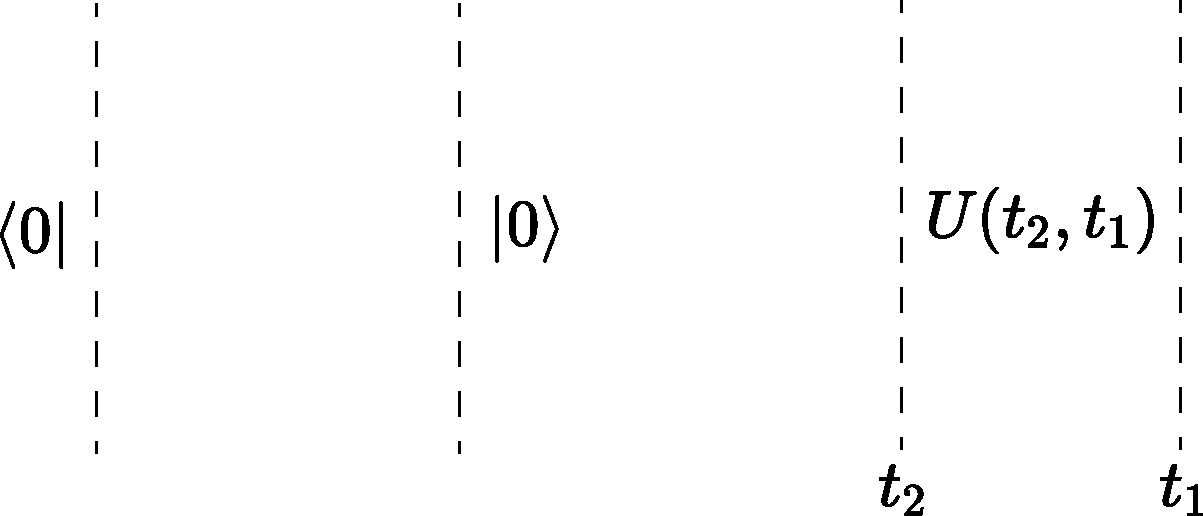
\includegraphics[width=0.5\hsize]{../images/time vacuum.pdf}
    \caption{真空状態と時間発展演算子の図式による表現}
\end{figure}
例えば$\^U(t_2,t_1)|0⟩ = |0⟩$という式は、
\begin{figure}[H]
    \centering
    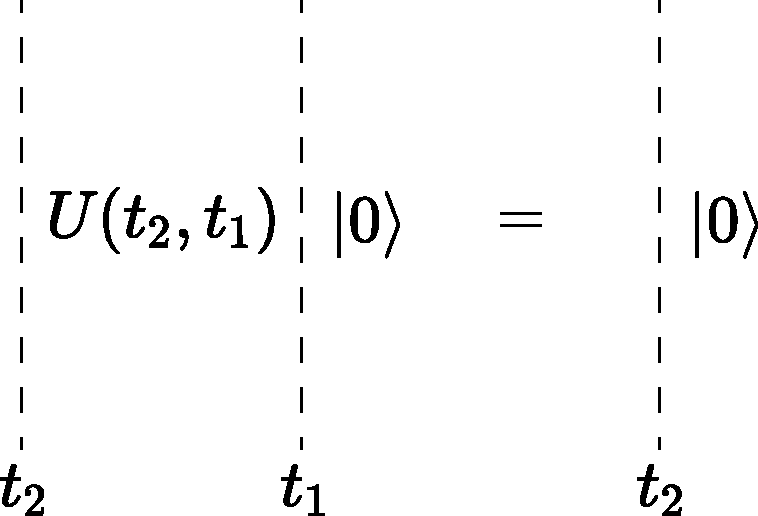
\includegraphics[width=0.3\hsize]{../images/U0 = 0.pdf}
    \caption{図式による計算}
\end{figure}
と図示できる。

\subsection{
    場の演算子と相関関数
}
Schr\"odinger表示の場の演算子$\^φ(𝒙)$を$|φ⟩$を固有状態にもつ演算子として、
\begin{align}
    \^φ(𝒙) ≔ ∫\𝒟φ φ(𝒙)|φ⟩⟨φ|,\␣
    \^φ(𝒙)|φ'⟩ = φ'(𝒙)
\end{align}
によって定義する。
Heisenberg表示での演算子は、
\begin{align}
    \^ϕ(t,𝒙) = \^U(0,t)\^φ(𝒙)\^U(t,0)
    \label{QFT: definition of ϕ operator}
\end{align}
と定義される。ここで、$t>t'$に対して$\^U(t',t)=\^U(t,t')^{-1}$と定義している。
Heisenberg表示では演算子の始域、終域は全て時刻$0$のHilbert空間に揃えられている。
これによって、Heisenberg表示では異なる時刻の演算子でも足し引きが問題なく定義できる。

相関関数を場の演算子によって表すことができる。
1点関数$\⟨ϕ(t,𝒙)\⟩$は、
\begin{align}
    ⟨ϕ(t,𝒙)⟩ &
    = \f{1}{Z}∫^{ϕ(t_\rm{f})=φ_\rm{f}}_{ϕ(t_\rm{i})=φ_\rm{i}}
        \𝒟{ϕ}ϕ(t,𝒙)\e^{-S[ϕ]}
    \∅ &
    = \f{1}{Z}∫\𝒟φ φ(𝒙)
    ∫^{ϕ(t_\rm{f})=φ_\rm{f}}_{ϕ(t)=φ}\𝒟{ϕ}
    ∫^{ϕ(t)=φ}_{ϕ(t_\rm{i})=φ_\rm{i}}\𝒟{ϕ}\e^{-S[ϕ]}
    \∅ &
    = \f{1}{Z}∫\𝒟φ ⟨φ_\rm{f}|\^U(t_\rm{f},t)|φ⟩φ(𝒙)⟨φ|\^U(t,t_\rm{i})|φ_\rm{i}⟩
    \∅ &
    = \f{
        ⟨φ_\rm{f}|\^U(t_\rm{f},t)\^φ(𝒙)\^U(t,t_\rm{i})|φ_\rm{i}⟩
    }{
        ⟨φ_\rm{f}|\^U(t_\rm{f},t_\rm{i})|φ_\rm{i}⟩
    }
    \∅ &
    = \f{
        ⟨φ_\rm{f}(t_\rm{f})|\^ϕ(x)|φ_\rm{i}(t_\rm{i})⟩
    }{
        ⟨φ_\rm{f}(t_\rm{f})|φ_\rm{i}(t_\rm{i})⟩
    }
    \label{one point function}
\end{align}
と表せる。ただし、状態のHeisenberg表示を
\begin{align}
    |φ(t)⟩ = \^U(0,t)|φ⟩
\end{align}
と定義した。
\footnote{
Heisenberg表示の状態が時間に依存していて違和感があるが、$|φ⟩$はHamiltonianに従って時間発展しているわけではないので、時間に依存してもよい。
}

無限大の領域での相関関数を考える場合、始状態・終状態を真空状態に変えれば良い。
まず、$\^H|0⟩=0$となるように作用の定数項を調節したとき、
\begin{align}
    Z = ⟨0|\^U(t_\rm{f},t_\rm{i})|0⟩ = 1
\end{align}
となることに注意すると、
\begin{align}
    ⟨ϕ(x)⟩ = ⟨0|\^ϕ(x)|0⟩
\end{align}
となる。

同様に2点関数は、$t₁ > t₂$のとき、
\begin{align}
    &
    ⟨ϕ(t₁,𝒙₁)ϕ(t₂,𝒙₂)⟩
    \∅ &
    = \f{1}{Z}∫\𝒟{φ₁}\𝒟{φ₂}φ₁(𝒙₁)φ₂(𝒙₂)
    ∫^{ϕ(t_\rm{f})=φ_\rm{f}}_{ϕ(t₁)=φ₁}\𝒟{ϕ}
    ∫^{ϕ(t₁)=φ₁}_{ϕ(t₂)=φ₂}\𝒟{ϕ}
    ∫^{ϕ(t₂)=φ₂}_{ϕ(t_\rm{i})=φ_\rm{i}}\𝒟{ϕ}
    \e^{-S[ϕ]}
    \∅ &
    % = \f{1}{Z}⟨φ_\rm{f}|
    % \^U(t_\rm{f},t₁)\^φ(𝒙₁)\^U(t₁,t₂)\^φ(𝒙₂)\^U(t₂,t_\rm{i})
    % |φ_\rm{i}⟩
    % \∅ &
    = \f{
        ⟨φ_\rm{f}(t_\rm{f})|
        \^ϕ(t₁,x₁)\^ϕ(t₂,x₂)
        |φ_\rm{i}(t_\rm{i})⟩
    }{
        ⟨φ_\rm{f}(t_\rm{f})|φ_\rm{i}(t_\rm{i})⟩
    }
\end{align}
と表せる。
途中式は(\ref{one point function})と同じなので省略した。
分子は以下のように図示できる。
\begin{figure}[H]
    \centering
    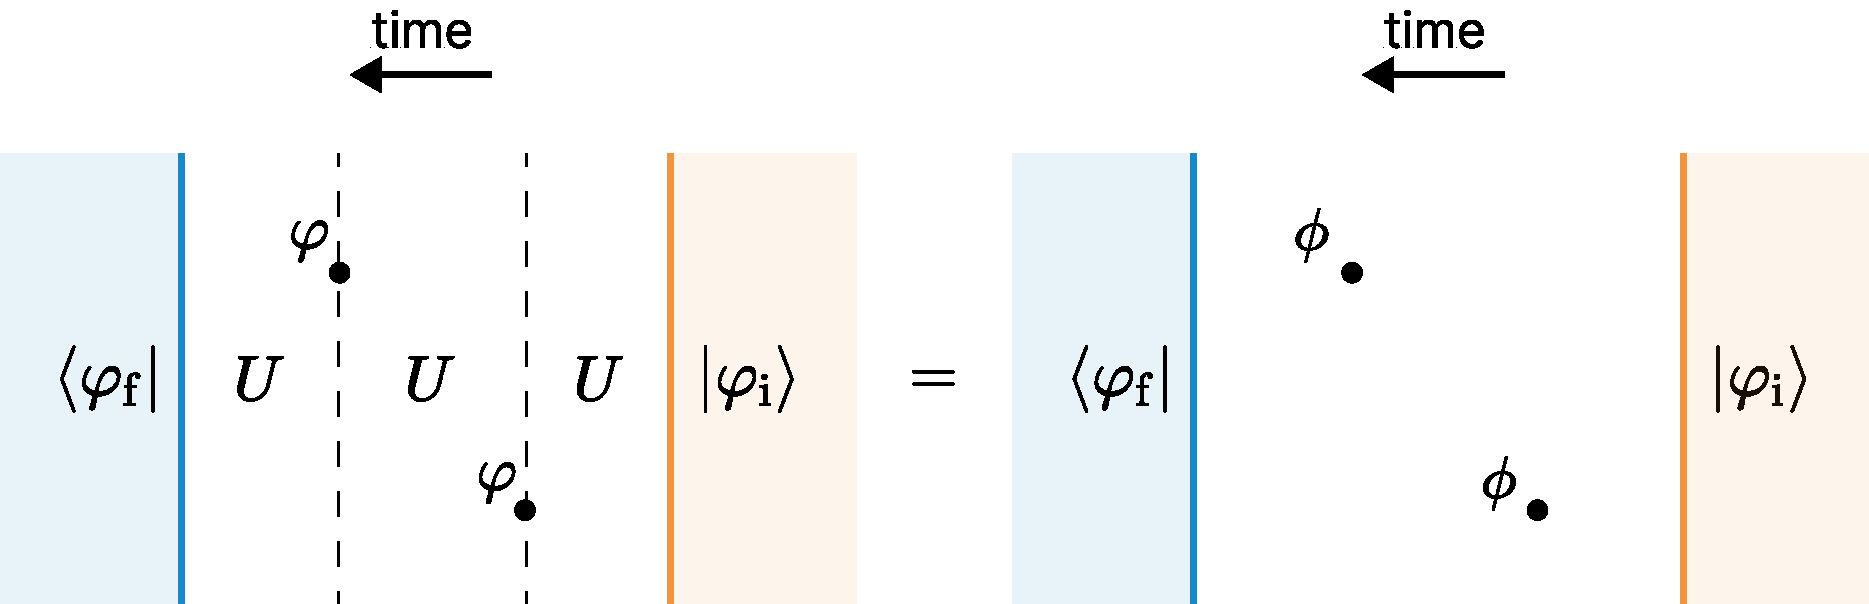
\includegraphics[width=0.7\hsize]{../images/two point function.pdf}
    \caption{2点関数}
\end{figure}
$t₁ < t₂$のときは$\^ϕ(t₁,𝒙₁)$と$\^ϕ(t₂,𝒙₂)$の順序を入れ替える必要があるので、
\begin{align}
    \⟨ϕ(x₁)ϕ(x₂)\⟩
    = \f{
        ⟨φ_\rm{f}(t_\rm{f})|𝖳^*{\Q[\^ϕ(x₁)\^ϕ(x₂)]}|φ_\rm{i}(t_\rm{i})⟩
    }{
        ⟨φ_\rm{f}(t_\rm{f})|φ_\rm{i}(t_\rm{i})⟩
    }
\end{align}
となる。$𝖳^*$積は左側が未来、右側が過去になるように演算子を並べて積をとることを表す。
\footnote{
    $𝖳^*$積と類似の概念で$𝖳$積というのがあるので違いを説明しておく。$𝖳$積は、
    \begin{align}
        𝖳\l[\^ϕ(x₁)\^ϕ(x₂)\r]
        = \^ϕ(x₁)\^ϕ(x₂)θ(t₁-t₂)+\^ϕ(x₂)\^ϕ(x₁)θ(t₂-t₁)
    \end{align}
    と定義される。一方$𝖳^*$積は相関関数から定義される。
    演算子の時間微分が含まれていない場合、$𝖳$積と$𝖳^*$積は同じ結果を与える。
    \begin{align}
        \⟨ϕ(x₁)ϕ(x₂)\⟩
        = ⟨0|𝖳^*\l[\^ϕ(x₁)\^ϕ(x₂)\r]|0⟩
        = ⟨0|𝖳\l[\^ϕ(x₁)\^ϕ(x₂)\r]|0⟩
    \end{align}
    時間微分が含まれる場合、$𝖳^*$積は相関関数から定義されるので、時間微分は期待値の外に出すことができ、
    \begin{align}
        &
        ⟨0|𝖳^*\l[∂₀\^ϕ(x₁)\^ϕ(x₂)\r]|0⟩
        =\∂{t₁}⟨0|𝖳\l[ϕ(x₁)ϕ(x₂)\r]|0⟩
        \∅ &
        = ⟨0|𝖳\l[∂₀\^ϕ(x₁)\^ϕ(x₂)\r]|0⟩
        + ⟨0|\l[\^ϕ(x₁),\^ϕ(x₂)\r]|0⟩δ(t₁-t₂)
    \end{align}
    となる。したがって$𝖳$積と$𝖳^*$積の間にはデルタ関数に比例する項の分の差があることがわかる。
}
始状態・終状態を真空にとると、
\begin{align}\tcboxmath{
    \⟨ϕ(x₁)ϕ(x₂)\⟩
    = ⟨0|𝖳^*{\Q[\^ϕ(x₁)\^ϕ(x₂)]}|0⟩
}\end{align}
となる。
同様に、$n$点関数について以下が成り立つ。
\begin{align}\tcboxmath{
    \⟨ϕ(x₁)⋯ϕ(xₙ)\⟩
    = ⟨0|𝖳^*{\l[\^ϕ(x₁)⋯\^ϕ(xₙ)\r]}|0⟩.
}\end{align}

\subsection{
    一般的な量子化
}
演算子形式の場の理論では、時間一定の超平面で時空をスライスし、その断面にHilbert空間を対応づける。
しかし、時空の切り方は一つではない。
回転対称な理論では時間の方向の取り方は任意であるし、時空を超曲面で切ることもできる。
時空を超曲面でスライスした場合も時間発展演算子や場の演算子を同様に定義することが可能である。
\begin{figure}[H]
    \centering
    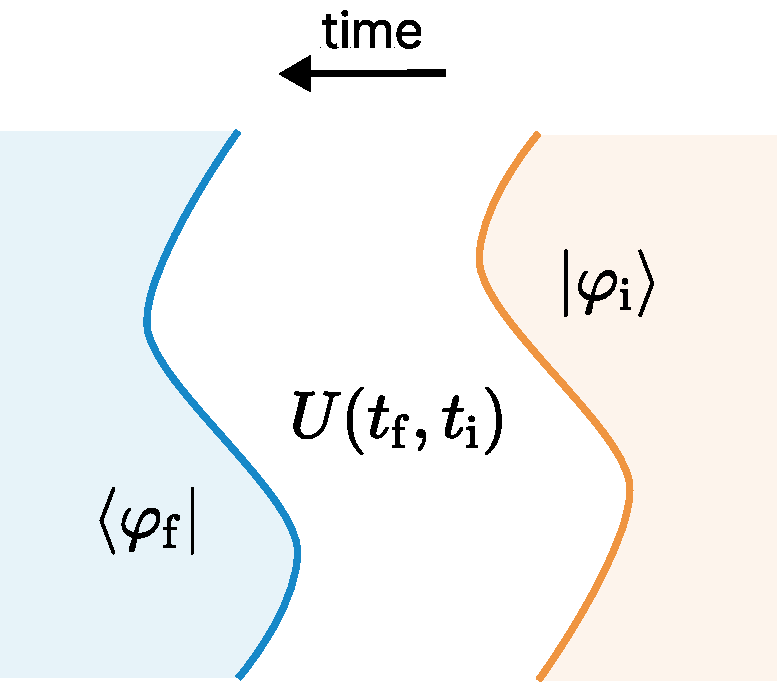
\includegraphics[width=0.3\hsize]{../images/general quantization.pdf}
    \caption{一般的な量子化}
\end{figure}
これは一般的すぎて机上の空論な感もあるが、共形場理論では動径量子化やN-S量子化など、平面で切らないような量子化で性質の良いものが存在する。
動径量子化は後で扱う。N-S量子化については\cite{Rychkov_2017}を参照してほしい。

また一方向に進む時間という概念にこだわらなければ、より拡張された形で演算子を定義できる。
未来と過去に境界条件をつけて行列要素を定義する場合、演算子$\^U(t_\rm{f},t)\^𝒪(𝒙)\^U(t,t_\rm{i})$は2つの時刻のHilbert空間$ℋ_{t_\rm{f}},ℋ_{t_\rm{i}}$の間の線型写像であるが、これを
\begin{align}
    𝒪(x): ℋ_{t_\rm{f}}⊗ℋ_{t_\rm{i}} → ℂ
\end{align}
とみなすこともできる。
この場合、$𝒪(x)$は境界条件に対して複素数を返す汎函数である。
ここで、一般的な局所演算子$𝒪(x)$を、$x$を含む領域の境界上で定義された場$φ$に対し、期待値$\⟨𝒪(x)\⟩_φ$を返す線形汎函数とみなせる。
\begin{align}
    𝒪(x): ℋ(∂B) → ℂ,~
    |φ⟩ ↦ ⟨𝒪(x)⟩_φ,\␣
    (x ∈ B)
\end{align}
\begin{figure}[H]
    \centering
    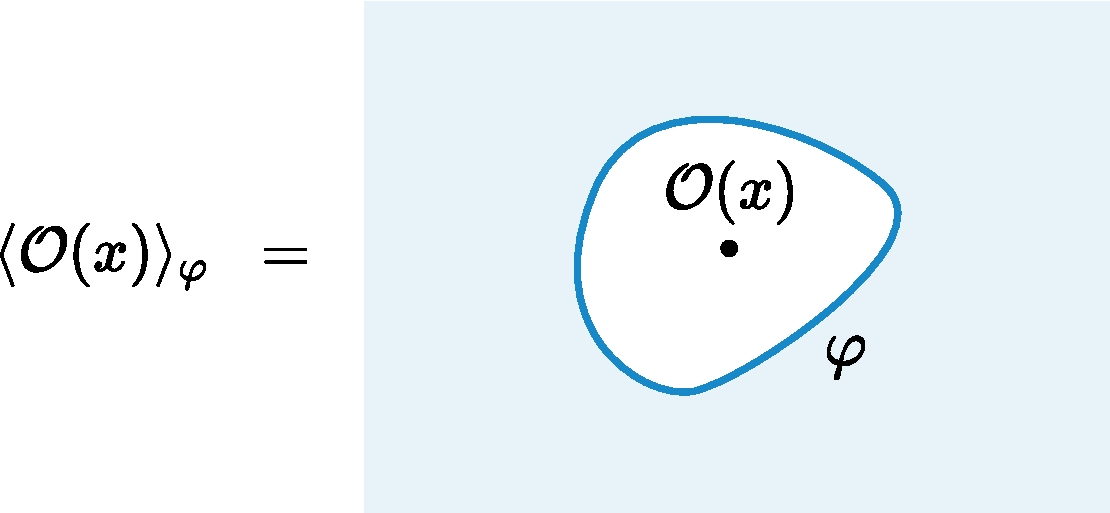
\includegraphics[width=0.4\hsize]{../images/general operator.pdf}
\end{figure}
経路積分に対する局所場の挿入はこの意味で演算子である。
また$∀φ,\⟨𝒪(x)\⟩_φ=\⟨𝒪'(x)\⟩_φ$となるとき、演算子の等式として$𝒪(x)=𝒪'(x)$と書くことにする。
この書き方は以降の議論で頻繁に用いる。
\end{document}